\label{sec:methods}
\section{Methods and Materials}

The design and the implementation of the nuclear reactor were carried out using MCNP5.1 run both locally, as well as remotely on servers to verify results.  The design was approached in a "bottom-up" faction. This meant that the reactor's core was designed and tested first. After this, the surrounding material, as well as its geometry, were designed and tested for optimal neutron reflectivity. Finally, the output chamber was added with an FMESH tally running the neutron counts. This approach allowed us to incrementally structure the reactor and catch any errors in their early stages.\\

\subsection{Core}

After considering several variations of breeder reactors, all of which were Thorium based, the element of choice for the core was Uranium-235. Due to safety concerns for real-life implementation, its purity could not be 100\%, however reactivity calculations were carried out to understand initial core sizes at this percentage. Uranium-235's value in core composition was decreased to 19\% after initial tests. Again, this was done to address safety concerns while operating the reactor. The rest of the core, mainly 81\%, was made up of Graphite for neutron moderation.\\

The core was designed in the following way. Two layers of Uranium-235 blocks are arranged in a 2 by 4 grid. In between each block and both layers, the Graphite acts as the neutron moderator. The structure can be seen in figure \ref{fig:core}.

\begin{figure}[!htbp]
\caption{Reactor core cross sections.}
\label{fig:core}
\centering
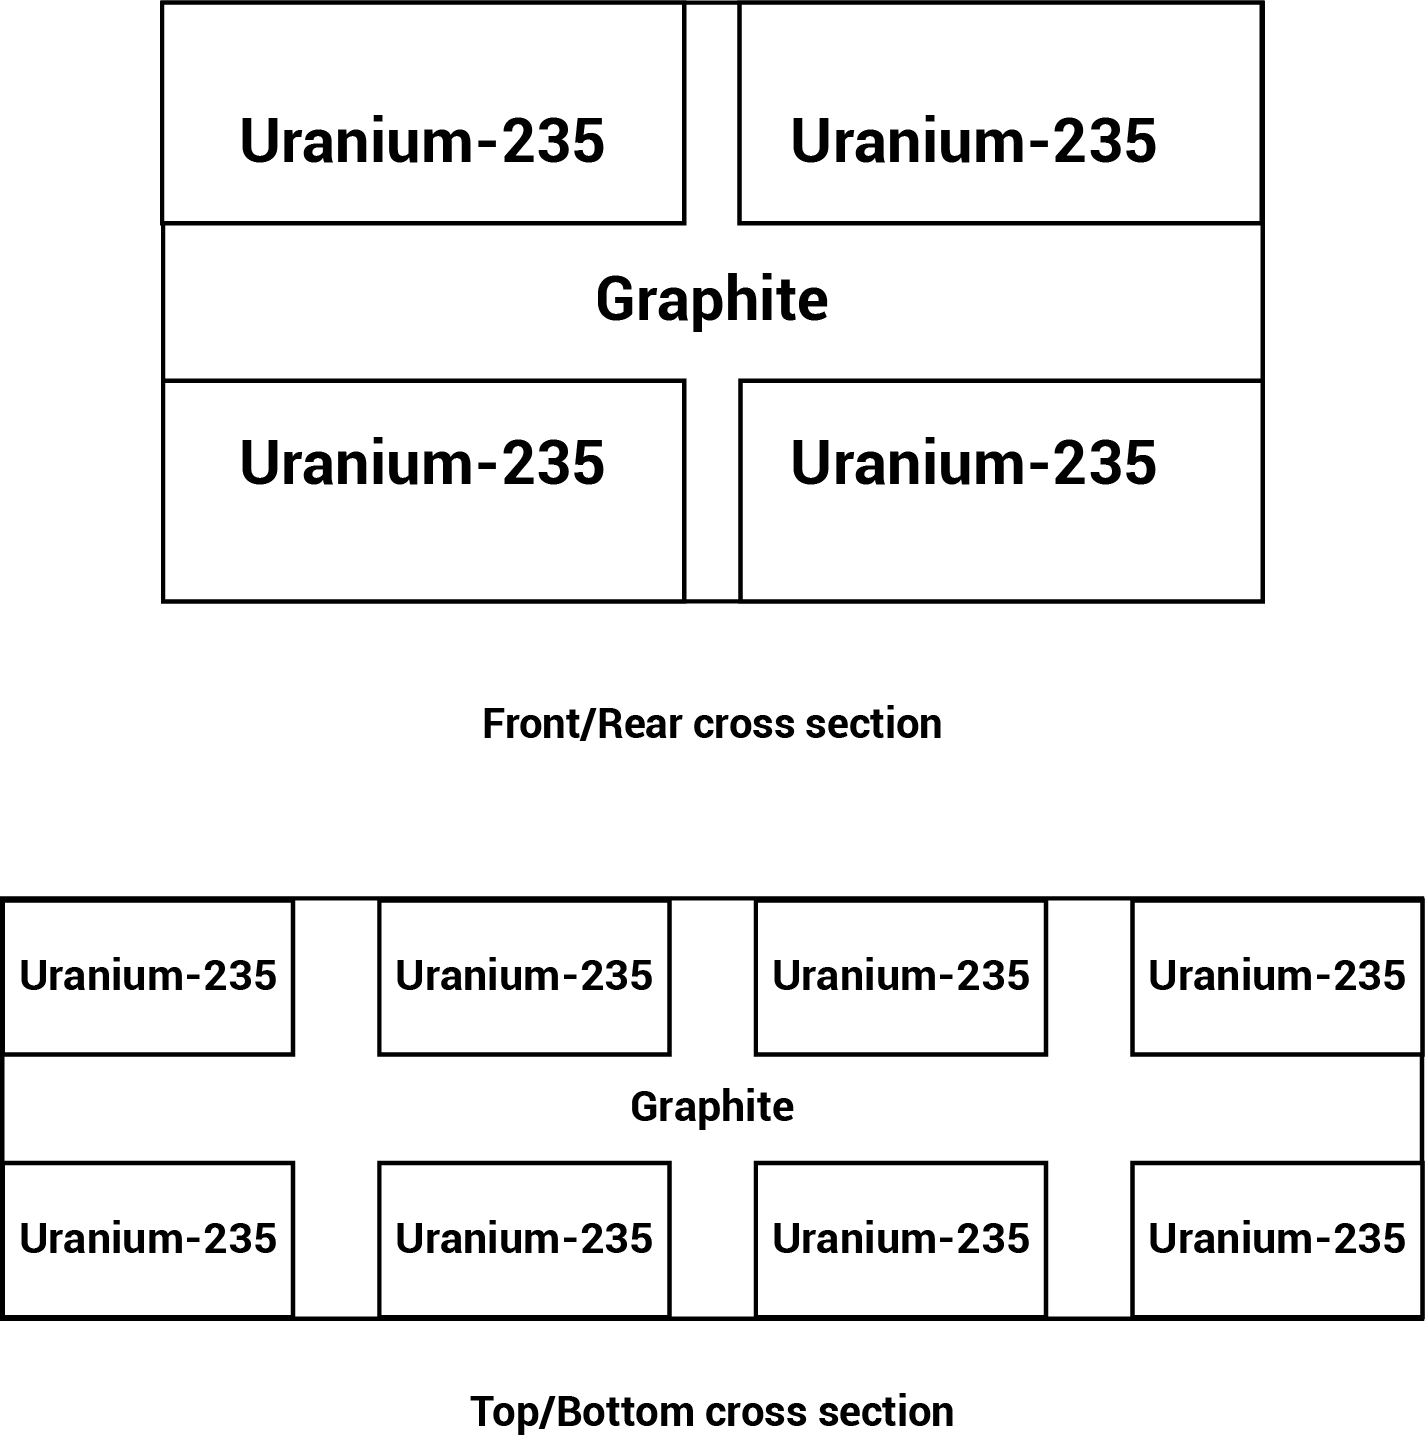
\includegraphics[width=0.75\textwidth]{core.png}
\end{figure}

With this structure, all of the emitted and absorbed neutrons will be regulated by the Graphite. The likelihood of a runaway reaction decreases due to the embedding of the Uranium blocks. For the reaction to be sustainable, the neutrons should be thermal, hence fast neutrons will not be captured and will not contribute to the fissions. Instead, they will be absorbed (along with excess particles) by the Graphite.\\

The structure of the core, however, can be simplified for the MCNP simulations and further power calculations. The complete block of Uranium and Graphite can be turned into one single block. As already stated, the composition of said block will be a 19\%-81\% split of Uranium-235 and Graphite. The dimensions and composition were chosen after running criticality simulations. More detailed information on the core's dimensions and criticalities can be found in section \ref{sec:results}.

\subsection{Shell}

The surrounding shell and its geometry have several purposes in the reactor:
\begin{enumerate}
	\item Neutron reflection. The neutrons that are emitted from the core need to not be lost after one interaction. As a result, the surrounding shell's geometry was optimized to increase reflectivity of particles back into the core. This closed system is able to maintain the reaction. The thermal neutrons will reflect off of the walls and be directed towards the reactor to trigger further fissions.
	\item Thermal regulation. Any heat given off by the fission reactions needs to be transported out of the system to control the temperature. This is outside the scope of the project, however, some discussion is given in section \ref{sec:future}.
	\item Particle interaction. This is a middle ground between the previous two purposes. The material that the core is submerged in plays an important role in particle interaction. Materials looked at were water, graphite and vacuum.
\end{enumerate}

\subsubsection{Neutron reflection}

An already existing example of reflection was taken into account when looking at the shell's neutron reflection capabilities - a parabolic dish. A ray diagram of how a parabolic reflector works can be seen in figure \ref{fig:parabola}.

\begin{figure}[!htbp]
\caption{Parabolic reflector.}
\label{fig:parabola}
\centering
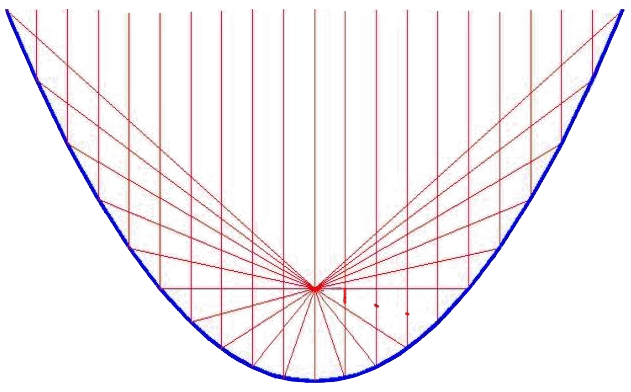
\includegraphics[width=0.75\textwidth]{parabola.png}
\end{figure}

From this, a circular design of the shell was implemented for initial simulations, with the reactor core in the middle. However, looking at the structure presented in figure \ref{fig:structure}, a problem arose with neutron direction.

\begin{figure}[!htbp]
\caption{Core and shell structures.}
\label{fig:structure}
\centering
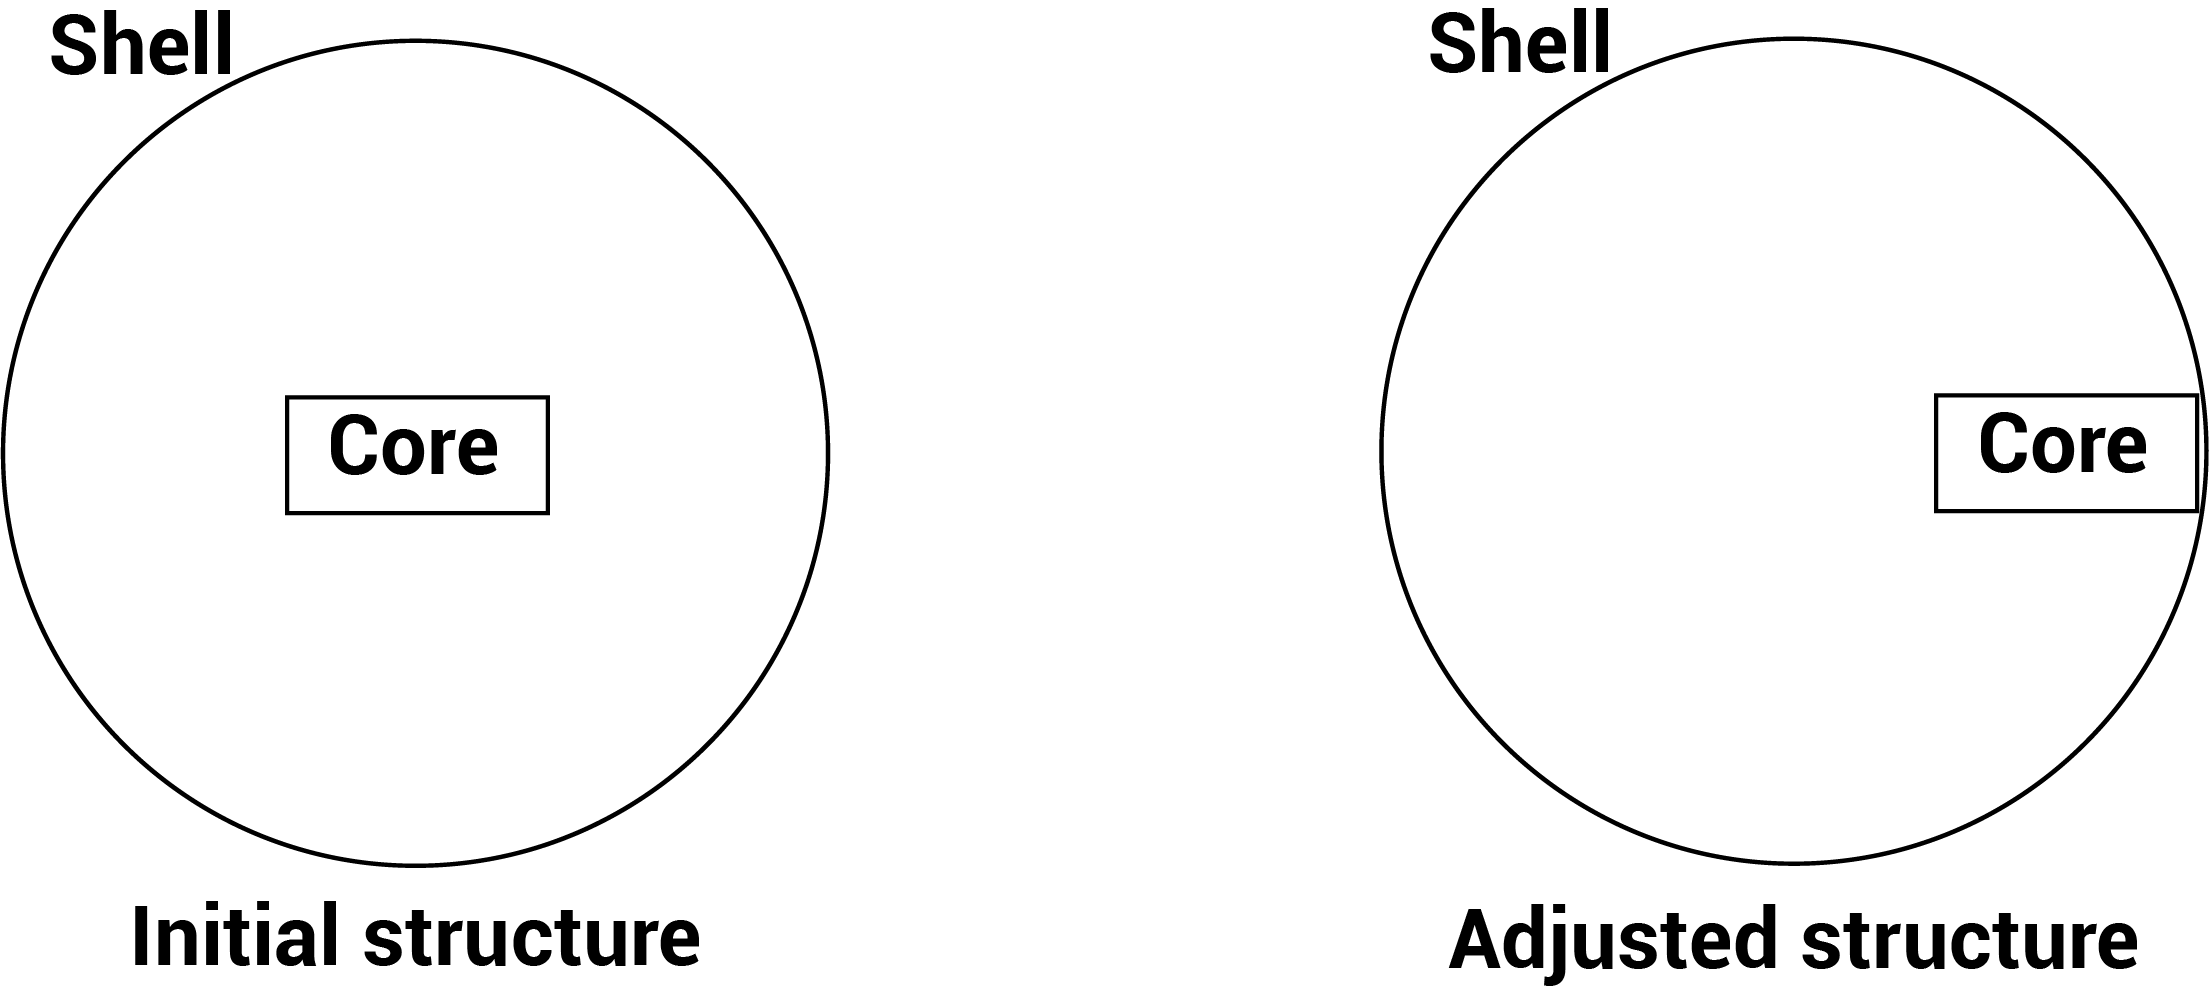
\includegraphics[width=0.75\textwidth]{structure.png}
\end{figure}

Neutrons that are to be used in research would be extremely difficult to direct towards an opening. Whatever directing structure that had to be added to the geometry would interfere with the parabolic reflective properties. As a result, a decision was made to move the core to one edge of the shell, seen under "Adjusted structure" in figure \ref{fig:structure}.

\subsubsection{Particle interaction}

Several materials were looked at with which to fill the shell around the core. These were water, graphite and vacuum. Looking at the criticality results in section \ref{sec:results}, using water enabled a criticality coefficient of $k\approx 1$. This meant that the core was perfectly critical - with little chances of creating a runaway chain reaction or the fission reactions dying out. Vacuum did not interact with the neutrons at all, which may have created issues later on with sustained reactions. Graphite has been omitted since the k-coefficient value was over 2, indicating an extremely volatile and supercritical core.
\subsection{Chamber}

With the core shifted to the side of the enclosing shell, it was now possible to add the neutron chamber on that very side. One side of the core's structure would be directly exposed to the chamber. As a result, the neutrons produced on that side would be emitted directly for flux calculations and use. The other 5 sides of the rectangular core structure would be fueling the fission reactions through the emission and reflection of thermal neutrons within the shell itself. From the criticality results, seen in section \ref{sec:results}, the side length of the core was taken to be $12cm$ in each direction. From this we see that the core is actually a cube. As a result, the cross section of the chamber is 12x12cm in order to capture all particles emitted. The placement of the core reduces particle leak, however, due to the nature of the geometry (cube placed against a spherical surface), some neutrons may leak back into the shell. The flux lost due to this is negligible since the returned neutrons will fuel further fission reactions after being reflected back into the core by the shell.
\subsection{Tally}